\paragraph{QuizziPedia::Front-End::Views::ResultsQuestionnarieView}
\begin{figure} [ht]
	\centering
	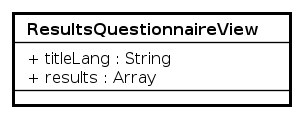
\includegraphics[scale=0.80]{UML/Classi/Front-End/QuizziPedia_Front-end_ResultsQuestionnarieView.png}
	\caption{QuizziPedia::Front-End::Views:ResultsQuestionnarieView}
\end{figure} \FloatBarrier
\begin{itemize}
	\item \textbf{Descrizione}: view contenente i risultati conseguiti dagli utenti che hanno compilato il proprio questionario;
	\item \textbf{Utilizzo}: permette di visualizzare i risultati di ogni utente conseguiti nella compilazione del questionario;
	\item \textbf{Relazioni con altre classi}:
	\begin{itemize}
		\item \textit{IN} \texttt{ResultsController}: questa classe permette di gestire i risultati della ricerca effettuata dall'utente;
		\item \textit{IN} \texttt{ResultsQuestionnaireModelView}: classe di tipo modelview la cui istanzazione è contenuta all'interno della variabile di ambiente \$scope di \texttt{Angular.js}. All'interno di essa sono presenti le variabili e i metodi necessari per il \textit{Two-Way Data-Binding\ped{G}} tra la view \texttt{ResultsQuestionnarieView} e il controller \texttt{ResultsController}; 
		\item \textit{IN} \texttt{LangModel}: rappresenta il modello delle informazioni per la giusta traduzione dell'applicazione.
	\end{itemize}
	\item \textbf{Attributi}:
	\begin{itemize}
		\item \texttt{+ titleLang: String} \\ Attributo che viene utilizzato per visualizzare la giusta traduzione del titolo della pagina, in italiano o in inglese; 
		\item \texttt{+ results: Array} \\ Array contenente un oggetto per ogni iscritto che ha compilato il questionario. L'oggetto sarà composto dai campi: \texttt{nome} e \texttt{cognome} e \texttt{valutazione}.
	\end{itemize}
\end{itemize}